\documentclass{article}
\usepackage{xcolor, graphicx}
\usepackage{mathabx}
\usepackage{hyperref}
\hypersetup{colorlinks=false}
\author{Edderic Ugaddan}
\title{Granuvolver}
\begin{document}
	\maketitle
	\tableofcontents
	\section{Gratitude}

	Special thanks goes to Dr. Benjamin Broening and Dr. Barry Lawson. First of all, thank you for being wonderful top-notch professors. I've really enjoyed all my classes with you, learning from you, and having one-on-ones with you, no matter how stressful it was at times. Thank you for helping me create my interdisciplinary major, Computer Music, and taking me under your wings as an advisee, giving me advice and showing me a different way to look at things whenever I was getting too caught up with an idea.  In the end, I feel that I've become a much better programmer, musician, and most of all, person.

	\section{Introduction}

	The objective of this Computer Music interdisciplinary senior thesis is to explore the combination of Granular Synthesis and Convolution. This entails programming a custom-made Max for Live (M4L) MIDI instrument that combines the two technologies, analyzing the sounds that come out of this combination, and finally creating music using the resulting sounds as source material. Granular synthesis is the method of producing interesting, texturally rich sounds by overlaying grains, sets of samples that are about 100 ms. or less in length. Convolution describes the mathematical process of sliding multiplication of two signals.   To the knowledge of the author, no MIDI instrument has been made that is specifically made only for exploring the combining of these two technologies.


	\section{Granular Synthesis}
		\subsection{What is it?}
			Granular Synthesis is the creation of sound via means of aggregating various sets of samples called grains. A grain is defined as:
			\begin{quote} 
				\ldots a brief microacoustic event, with a duration near the threshold of human auditory perception, typically \ldots [being less than] one tenth of a second, serving as a building block for sound objects.\cite[Loc. 1024]{Curtis_gs_def} 
			\end{quote}

			It was largely inaccessible in the past due to technological limitations of analog circuitry and tape. However, thanks to the advances in computing and hardware, composers are now able to digitalize audio and work with the latter in a sample-by-sample basis, thereby letting composers explore the "extreme limits of perception and performance."\cite[Loc. 334]{Curtis_gs}  Combining these grains helps us create animated, texturally rich sonic atmospheres.\cite[Loc. 1024]{Curtis_gs_def}    
			
	\section{Convolution}
		\subsection{What is it?}
			Convolution, in digital signal processing, is the mathematical process of sliding and overlapping two signals together, point-wise multiplying the coefficients, and summing the products. In more mathematically-precise terms, 

		\begin{equation}
			(f \convolution g) = \sum_{m=-\infty}^{\infty} f[m] g[n-m] 
		\end{equation} 
		where $f$ and $g$ are the two signals being convolved.\cite[121]{JOS_conv}  

		\subsection{Reverberation}

			Convolution, amongst music producers, is most famous for simulating the reverberation of physical spaces by a sound object.  For example, consider recording a drum that is hit in a small room, and then recording the reverberation of a large concert hall (stimulated by a quick transient such as a loud clap).  Convolving the two signals results in a "smearing"; the transient of the drum hit is smeared by the long reverb tail of the concert hall. The acoustical result would sound as if the drum hit was played in the large concert hall.

		\subsection{Algorithmic Efficiency}

			The naive implementation, which is called "direct" convolution, has a time efficiency of $O(n^2)$, where $n$ is the number of samples. This is terribly inefficient, considering that $n$ is quite large even for a small amount of time--the standard CD-quality audio signal has a sampling rate of 44.1 kHz (three seconds of recording, for example, would amount to greater than $10^5$ samples, and the resulting floating-point operations for convolution would be in the order of $10^{10}$).  

			Performing the Fast Fourier Transform (FFT), the point-wise multiplication, and the accompanying inverse FFT of the two signals shaves the time complexity to $O(n$log$n)$. A \emph{drastic} improvement indeed.  However, since $n$ is quite large, the convolution will still incur lots of latency and thus cannot be considered "real-time."  More complicated FFT algorithms take advantage of the audio signals' \emph{linearity} to speed up the convolution process. Partitioning the signals and doing many smaller FFTs in parallel helps decrease latency to the point of making it usable for real-time convolution.\cite{Batten_conv} Dr. Alex Harker's real-time implementation, called $multiconvolve$\~{}, is a Max/MSP object that is used in this thesis to help speed up the music making process.\cite{pa}


	\section{Granuvolver}
		\subsection{Why Max?}
		Granuvolver was originally made using the cross-platform Virtual Studio Effect (VST) SDK using C++. VST, developed by Steinberg, Inc. is a very popular audio plugin format that is supported by major Digital Audio Workstations (DAWs), such as Logic, Ableton Live, Cubase, ProTools, and Reaper.  Unfortunately, implementing VSTs is not trivial. VST SDKs do not come with built-in audio effects or GUI elements. Also one can easily get stuck working more on IDE configuration settings than on actual programming. See section on  \href{http://teragonaudio.com/article/How-to-make-VST-plugins-in-Visual-Studio.html}{build settings for Visual Studio}, for example.

		Max, a proprietary software developed by Cycling 74, is a graphical, programmable, patching environment written in C.  Objects have inlets and outlets that one can connect to other objects. One can create more powerful objects by making one that is composed of many built-in objects. One can also create external objects in Javascript and Java very easily. However, if one wants more efficient performance and does not mind doing manual garbage collection, one can even develop externals in pure C, C++, and even in Objective-C. Unfortunately, a regular undiscounted license is a hefty \$399.

		Yet, Max ultimately became the final implementation environment solely for several reasons. First, it allows fast prototyping. Max (vers. 6.1) has over 1,000 native objects that can be quickly used, such as objects for dropping (and recognizing paths) of audio files, displaying waveforms and selecting sections of the waveforms, and filtering an incoming audio signal. By providing easily editable and usable GUI elements and providing DSP objects, one can really put more time into actual music production and less into development. Second, users can develop Max for Live (M4L) objects, which can be easily and seamlessly patched, edited, and used within powerful Ableton Live 9 software for further editing and processing.
		\subsection{Features}
			\begin{enumerate}
				\item Stereo-based granulation of audio signals.
				\item Granulator uses Gaussian Normal Distribution with editable mean and pseudo-width to stochastically pick the next area to iterate.
				\item Subtractive synthesis (using a combo of low-pass and high-pass filters)
				\item Slope of curves of amplitude envelope are editable.
				\item Granulation of a signal can then be recorded into buffer to be used for \ldots
				\item Real-time convolution of the granulated signals.

			\end{enumerate}
		\subsection{Installation}

		\subsection{How to use}
			\begin{figure}[h!]
		  \centering
	    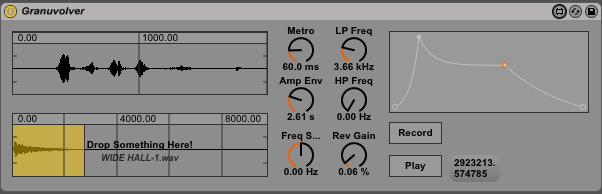
\includegraphics[width=1\textwidth]{images/Granuvolver}
		  \caption{Granuvolver}
			\end{figure}


		\subsection{Future Improvements}
			\subsubsection{Known Bugs}
			\subsubsection{Suggested Improvements}
	\section{Music Piece}
	\section{Conclusion}
	\section{References}
		\begin{thebibliography}{99}
		\bibitem{Curtis_gs_def} C. Roads, The History of Microsound, in \emph{Microsound}, 1st ed. Massachusetts, MIT Press, 2004, ch. 2, loc. 1024/4377 (Kindle), ISBN 0262182157

		\bibitem{Curtis_gs} C. Roads, Granular Synthesis, in \emph{Microsound}, 1st ed. Massachusetts, MIT Press, 2004, ch. 2, loc. 272/4377 (Kindle), ISBN 0262182157

		\bibitem{JOS_conv} Smith, J.O., Chapter 7: Fourier Theorems for the DFT. The Mathematics of the Discrete Fourier Transform (DFT) with Audio Applications. W3K Publishing, pp. 121. ISBN 9780974560748

		\bibitem{Batten_conv} Battenberg, Eric. et. al. Advances in the Parallelization of Music and Audio Applications. The Center for New Music and Audio Technologies and The Parallel Computing Laboratory, University of California Berkeley (2010)

		\bibitem{pa} Harker, Alexander and Tremblay, Pierre Alexandre (2012) The HISSTools Impulse Response Toolbox: Convolution for the Masses. In: ICMC 2012: Non-cochlear Sound. The International Computer Music Association, pp. 148-155. ISBN 9780984527410
		\end{thebibliography}
\end{document}